\documentclass{standalone}
\usepackage{tikz}
\usetikzlibrary{patterns, positioning}


\begin{document}
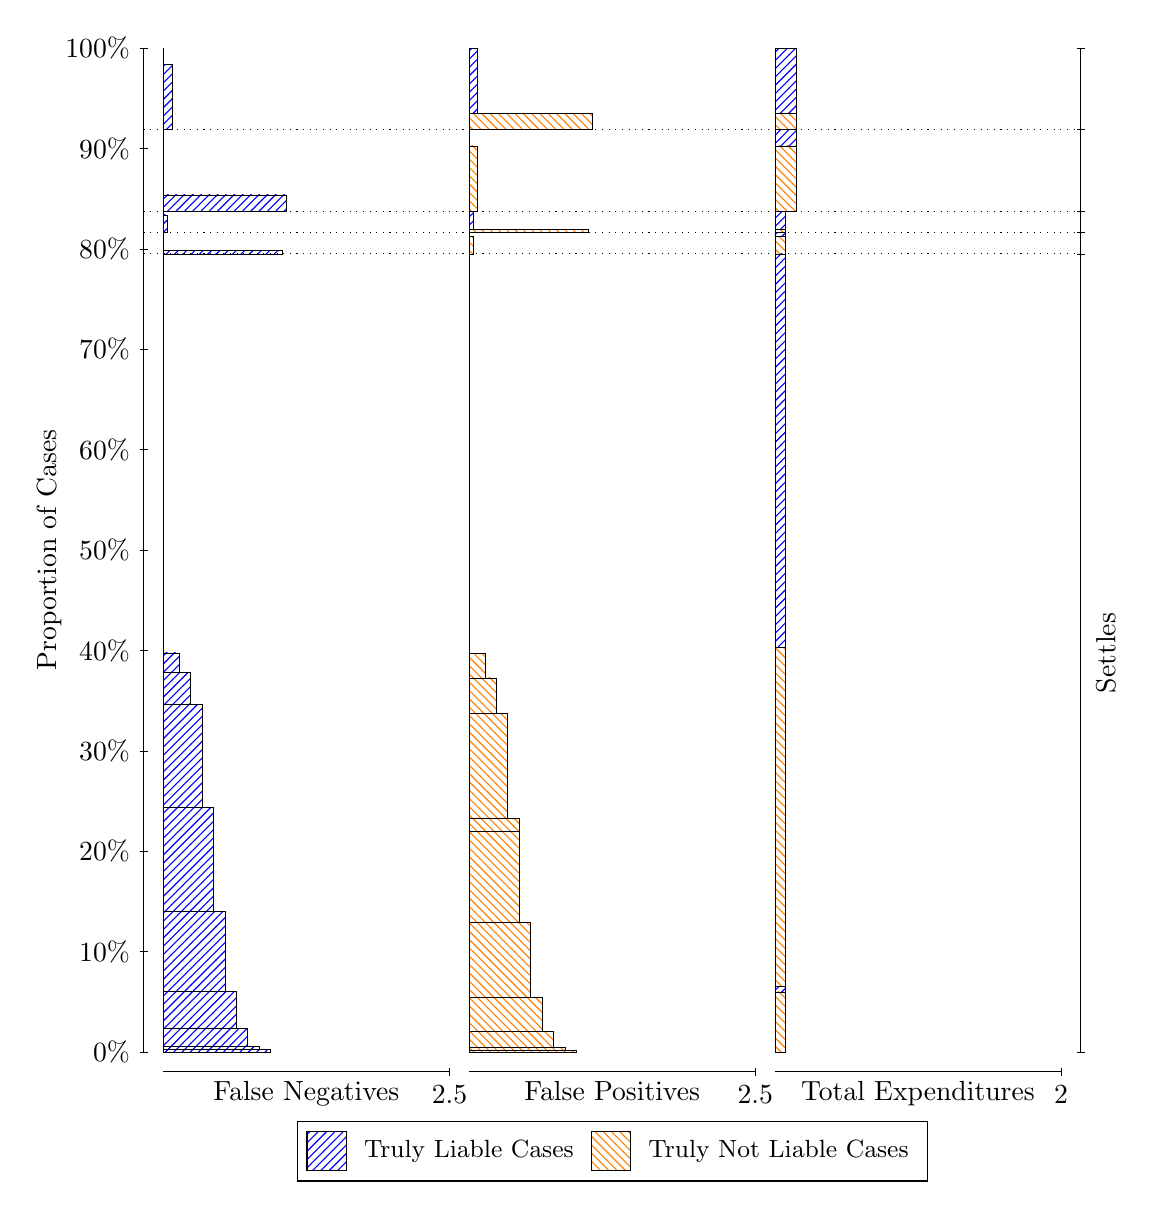
\begin{tikzpicture}
\draw[black, very thin] (1.5,1.75) -- (1.5,14.5);
\node[rotate=90, text=black, anchor=center] at (0.3, 8.125) {Proportion of Cases};
\draw[black, very thin] (1.45,1.75) -- (1.55,1.75);
\node[text=black, anchor=east] at (1.45, 1.75) {0\%};
\draw[black, very thin] (1.45,3.025) -- (1.55,3.025);
\node[text=black, anchor=east] at (1.45, 3.025) {10\%};
\draw[black, very thin] (1.45,4.3) -- (1.55,4.3);
\node[text=black, anchor=east] at (1.45, 4.3) {20\%};
\draw[black, very thin] (1.45,5.575) -- (1.55,5.575);
\node[text=black, anchor=east] at (1.45, 5.575) {30\%};
\draw[black, very thin] (1.45,6.85) -- (1.55,6.85);
\node[text=black, anchor=east] at (1.45, 6.85) {40\%};
\draw[black, very thin] (1.45,8.125) -- (1.55,8.125);
\node[text=black, anchor=east] at (1.45, 8.125) {50\%};
\draw[black, very thin] (1.45,9.4) -- (1.55,9.4);
\node[text=black, anchor=east] at (1.45, 9.4) {60\%};
\draw[black, very thin] (1.45,10.675) -- (1.55,10.675);
\node[text=black, anchor=east] at (1.45, 10.675) {70\%};
\draw[black, very thin] (1.45,11.95) -- (1.55,11.95);
\node[text=black, anchor=east] at (1.45, 11.95) {80\%};
\draw[black, very thin] (1.45,13.225) -- (1.55,13.225);
\node[text=black, anchor=east] at (1.45, 13.225) {90\%};
\draw[black, very thin] (1.45,14.5) -- (1.55,14.5);
\node[text=black, anchor=east] at (1.45, 14.5) {100\%};

\draw[black, very thin] (13.4,1.75) -- (13.4,14.5);
\draw[black, very thin] (13.35,1.75) -- (13.45,1.75);
\node[anchor=west] at (13.35, 1.75) {};
\draw[black, very thin] (13.35,11.885) -- (13.45,11.885);
\node[anchor=west] at (13.35, 11.885) {};
\draw[black, very thin] (13.35,12.156) -- (13.45,12.156);
\node[anchor=west] at (13.35, 12.156) {};
\draw[black, very thin] (13.35,12.427) -- (13.45,12.427);
\node[anchor=west] at (13.35, 12.427) {};
\draw[black, very thin] (13.35,13.465) -- (13.45,13.465);
\node[anchor=west] at (13.35, 13.465) {};
\draw[black, very thin] (13.35,14.5) -- (13.45,14.5);
\node[anchor=west] at (13.35, 14.5) {};

\draw[black, very thin, pattern color=blue, pattern=north east lines] (1.75,1.75) rectangle (3.1125,1.7782);
\draw[black, very thin, pattern color=blue, pattern=north east lines] (1.75,1.7782) rectangle (2.9672,1.8227);
\draw[black, very thin, pattern color=blue, pattern=north east lines] (1.75,1.8227) rectangle (2.8218,2.0538);
\draw[black, very thin, pattern color=blue, pattern=north east lines] (1.75,2.0538) rectangle (2.6765,2.5227);
\draw[black, very thin, pattern color=blue, pattern=north east lines] (1.75,2.5227) rectangle (2.5312,3.5342);
\draw[black, very thin, pattern color=blue, pattern=north east lines] (1.75,3.5342) rectangle (2.3858,4.8593);
\draw[black, very thin, pattern color=blue, pattern=north east lines] (1.75,4.8593) rectangle (2.2405,6.1663);
\draw[black, very thin, pattern color=blue, pattern=north east lines] (1.75,6.1663) rectangle (2.0952,6.5675);
\draw[black, very thin, pattern color=blue, pattern=north east lines] (1.75,6.5675) rectangle (1.9498,6.8181);
\draw[black, very thin, pattern color=orange, pattern=north west lines] (1.75,6.8181) rectangle (1.75,11.885);
\draw[black, very thin, pattern color=blue, pattern=north east lines] (1.75,11.885) rectangle (3.2578,11.929);
\draw[black, very thin, pattern color=orange, pattern=north west lines] (1.75,11.929) rectangle (1.75,12.156);
\draw[black, very thin, pattern color=blue, pattern=north east lines] (1.75,12.156) rectangle (1.8045,12.382);
\draw[black, very thin, pattern color=orange, pattern=north west lines] (1.75,12.382) rectangle (1.75,12.427);
\draw[black, very thin, pattern color=blue, pattern=north east lines] (1.75,12.427) rectangle (3.3123,12.635);
\draw[black, very thin, pattern color=orange, pattern=north west lines] (1.75,12.635) rectangle (1.75,13.465);
\draw[black, very thin, pattern color=blue, pattern=north east lines] (1.75,13.465) rectangle (1.859,14.292);
\draw[black, very thin, pattern color=orange, pattern=north west lines] (1.75,14.292) rectangle (1.75,14.5);
\draw[black, very thin, pattern color=orange, pattern=north west lines] (5.6333,1.75) rectangle (6.9958,1.7725);
\draw[black, very thin, pattern color=orange, pattern=north west lines] (5.6333,1.7725) rectangle (6.8505,1.8105);
\draw[black, very thin, pattern color=orange, pattern=north west lines] (5.6333,1.8105) rectangle (6.7052,2.0149);
\draw[black, very thin, pattern color=orange, pattern=north west lines] (5.6333,2.0149) rectangle (6.5598,2.4414);
\draw[black, very thin, pattern color=orange, pattern=north west lines] (5.6333,2.4414) rectangle (6.4145,3.3981);
\draw[black, very thin, pattern color=orange, pattern=north west lines] (5.6333,3.3981) rectangle (6.2692,4.5476);
\draw[black, very thin, pattern color=orange, pattern=north west lines] (5.6333,4.5476) rectangle (6.2692,4.7119);
\draw[black, very thin, pattern color=orange, pattern=north west lines] (5.6333,4.7119) rectangle (6.1238,6.054);
\draw[black, very thin, pattern color=orange, pattern=north west lines] (5.6333,6.054) rectangle (5.9785,6.4999);
\draw[black, very thin, pattern color=orange, pattern=north west lines] (5.6333,6.4999) rectangle (5.8332,6.8164);
\draw[black, very thin, pattern color=blue, pattern=north east lines] (5.6333,6.8164) rectangle (5.6333,11.885);
\draw[black, very thin, pattern color=orange, pattern=north west lines] (5.6333,11.885) rectangle (5.6878,12.111);
\draw[black, very thin, pattern color=blue, pattern=north east lines] (5.6333,12.111) rectangle (5.6333,12.156);
\draw[black, very thin, pattern color=orange, pattern=north west lines] (5.6333,12.156) rectangle (7.1412,12.2);
\draw[black, very thin, pattern color=blue, pattern=north east lines] (5.6333,12.2) rectangle (5.6878,12.427);
\draw[black, very thin, pattern color=orange, pattern=north west lines] (5.6333,12.427) rectangle (5.7423,13.257);
\draw[black, very thin, pattern color=blue, pattern=north east lines] (5.6333,13.257) rectangle (5.6333,13.465);
\draw[black, very thin, pattern color=orange, pattern=north west lines] (5.6333,13.465) rectangle (7.1957,13.673);
\draw[black, very thin, pattern color=blue, pattern=north east lines] (5.6333,13.673) rectangle (5.7423,14.5);
\draw[black, very thin, pattern color=orange, pattern=north west lines] (9.5167,1.75) rectangle (9.6529,2.5125);
\draw[black, very thin, pattern color=blue, pattern=north east lines] (9.5167,2.5125) rectangle (9.6529,2.5852);
\draw[black, very thin, pattern color=orange, pattern=north west lines] (9.5167,2.5852) rectangle (9.6529,6.8892);
\draw[black, very thin, pattern color=blue, pattern=north east lines] (9.5167,6.8892) rectangle (9.6529,11.885);
\draw[black, very thin, pattern color=orange, pattern=north west lines] (9.5167,11.885) rectangle (9.6529,12.111);
\draw[black, very thin, pattern color=blue, pattern=north east lines] (9.5167,12.111) rectangle (9.6529,12.156);
\draw[black, very thin, pattern color=orange, pattern=north west lines] (9.5167,12.156) rectangle (9.6529,12.2);
\draw[black, very thin, pattern color=blue, pattern=north east lines] (9.5167,12.2) rectangle (9.6529,12.427);
\draw[black, very thin, pattern color=orange, pattern=north west lines] (9.5167,12.427) rectangle (9.7892,13.257);
\draw[black, very thin, pattern color=blue, pattern=north east lines] (9.5167,13.257) rectangle (9.7892,13.465);
\draw[black, very thin, pattern color=orange, pattern=north west lines] (9.5167,13.465) rectangle (9.7892,13.673);
\draw[black, very thin, pattern color=blue, pattern=north east lines] (9.5167,13.673) rectangle (9.7892,14.5);
\draw[black, dotted] (1.5,11.885) -- (13.4,11.885);
\draw[black, dotted] (1.5,12.156) -- (13.4,12.156);
\draw[black, dotted] (1.5,12.427) -- (13.4,12.427);
\draw[black, dotted] (1.5,13.465) -- (13.4,13.465);
\draw[black, very thin] (1.75,1.5) -- (5.3833,1.5);
\node[text=black, anchor=north] at (3.5667, 1.5) {False Negatives};
\draw[black, very thin] (5.3833,1.45) -- (5.3833,1.55);
\node[text=black, anchor=north] at (5.3833, 1.45) {2.5};

\draw[black, very thin] (5.6333,1.5) -- (9.2667,1.5);
\node[text=black, anchor=north] at (7.45, 1.5) {False Positives};
\draw[black, very thin] (9.2667,1.45) -- (9.2667,1.55);
\node[text=black, anchor=north] at (9.2667, 1.45) {2.5};

\draw[black, very thin] (9.5167,1.5) -- (13.15,1.5);
\node[text=black, anchor=north] at (11.333, 1.5) {Total Expenditures};
\draw[black, very thin] (13.15,1.45) -- (13.15,1.55);
\node[text=black, anchor=north] at (13.15, 1.45) {2};

\node[text=black, centered, rotate=90] at (13.72, 6.8173) {Settles};





\draw (7.449999999999999,1.5) node[draw=none] (baseCoordinate) {};
\begin{scope}[align=center]
        \matrix[scale=0.5, draw=black, below=0.5cm of baseCoordinate, nodes={draw}, column sep=0.1cm]{
            \node[rectangle, draw, minimum width=0.5cm, minimum height=0.5cm, pattern color=blue, pattern=north east lines] {}; &
            \node[draw=none, font=\small, text=black] (B) {Truly Liable Cases}; &
            \node[rectangle, draw, minimum width=0.5cm, minimum height=0.5cm, pattern color=orange, pattern=north west lines] {}; &
            \node[draw=none, font=\small, text=black] (B) {Truly Not Liable Cases}; \\
            };
\end{scope}

\end{tikzpicture}
\end{document}